\section{State estimation}\label{ch:state-estimation}
In this chapter the motivation for full state estimation is discussed. Secondly the concept of observability is discussed, a concept which will turn out to be very relevant to all observers that are to be used later. Starting with the single observer, that is constructed in this chapter. \textcolor{red}{update if stuff on eigenvalues is written}

\subsection{Motivation for full state estimation}
Let us first discuss why there is a need for state estimation, consider the continuous linear time invariant system
\begin{equation}\label{eqn:standard-noiseless-system}
    \dot{x}(t) = Ax(t) + Bu(t), \quad y(t) = Cx(t) + Du(t).
\end{equation}
The solution to this system can be written as
\begin{equation*}
    \begin{split}
        x(t) &= e^{tA}x_{0} + \int_{0}^{t}e^{(t-\tau)A}Bu(\tau)d\tau \\
        y(t) &= Ce^{tA}x_{0} + \int_{0}^{t}Ce^{(t-\tau)A}Bu(\tau)d\tau + Du(t).
    \end{split}
\end{equation*}
where $x_0 = x(0)$ \cite[Equation. 6.4]{Hespanha2018LinearTheory}. When there is no input, $u(t)=0$ for $t \geq 0$, system \eqref{eqn:standard-noiseless-system} reduces to
\begin{equation*}
    \dot{x}(t) = Ax(t), \quad y(t) = Cx(t)
\end{equation*}
which has the solution
\begin{equation}\label{eqn:zero-input-solution}
    x(t) = e^{tA}x_0, \quad y(t) = Ce^{tA}x_0.
\end{equation}
Let us now consider the definition of Lyapunov stability as in \cite[Th. 8.2]{Hespanha2018LinearTheory}, which states that a system is stable if and only if all the eigenvalues $\lambda_i,i=1,2,\dots,n$ of $A$ have strictly negative real parts. The matrix exponential in equation \eqref{eqn:zero-input-solution} computed by writing the matrix $A$ into its Jordan normal form $J=PAP^{-1}$, where $P$ is a change of basis matrix. The solution can then be written as 
\begin{equation}\label{eqn:jordan-form-exponential}
    x(t) = P^{-1}e^{tJ}Px_0
\end{equation}
\cite[Section 7.3]{Hespanha2018LinearTheory}. The matrix $J$ takes the following form
\begin{equation}\label{eqn:jordan-matrix}
    J =
    \begin{bmatrix}
        J_1 & 0 & \cdots & 0 \\
        0 & J_2 & \cdots & 0 \\
        \vdots & \vdots & \ddots & \vdots \\
        0 & 0 & \cdots & J_l \\
    \end{bmatrix}
\end{equation}
where each $J_i$ is a Jordan block that has the form
\begin{equation}\label{eqn:jordan-block}
    J_i = 
    \begin{bmatrix}
        \lambda_i & 1 & 0 & \cdots & 0 \\
        0 & \lambda_i & 1 & \cdots & 0 \\
        0 & 0 & \lambda_i & \cdots & 0 \\
        \vdots & \vdots & \vdots & \ddots & \vdots \\
        0 & 0 & 0 & \cdots & \lambda_i \\
    \end{bmatrix}, \quad i=1,2,\dots,l.
\end{equation}
The size of each Jordan block $J_i$ is determined by the algebraic and geometric multiplicities of the eigenvalues of matrix $A$. The algebraic multiplicity of an eigenvalue indicates the number of times an eigenvalue appears. Or in other words, the number of duplicate eigenvalues. The geometric multiplicity indicates the number of independent eigenvalues associated with a certain eigenvalue.  The number of Jordan blocks for each eigenvalue is equal to the geometric multiplicity of that eigenvalue. An eigenvalue with an algebraic multiplicity of $3$ and a geometric multiplicity of $2$ corresponds to one $1 \times 1$ and one $2 \times 2$ Jordan block \cite[Section 7.1] {Hespanha2018LinearTheory}.

Substituting equation \eqref{eqn:jordan-block} into \eqref{eqn:jordan-matrix} gives the full Jordan matrix. Which in turn can be substituted into equation \eqref{eqn:jordan-form-exponential}. Using the Equations as in \cite[Section 7.3]{Hespanha2018LinearTheory} shows that if all eigenvalues of $A$ have strictly negative real parts, $x \rightarrow 0$ as $t \rightarrow \infty$. A matrix that satisfies these requirements is also knows as a stability matrix or a stable matrix. 

\begin{example}\label{ex:stability-example}
    Let us take a closer look at the stability of the system presented in Example \ref{ex:system} and Equation \eqref{eqn:example-system}. The eigenvalues and eigenvectors of the matrix $A$ are as in Table \ref{tab:eigen-example-system}. $\lambda_1=\lambda_3$ and $\lambda_2=\lambda_4$ so the algebraic multiplicity of both eigenvalues is $2$. $\mathbf{v}_1=-\mathbf{v}_3$ and $\mathbf{v}_2=-\mathbf{v}_4$ so the geometric multiplicity of both eigenvalues is 1, since the eigenvectors are dependent on each other.
    \begin{table}[H]
        \centering
        \begin{tabular}{|c|c|c|c|c|}
           \toprule
           $i$ & $1$ & $2$ & $3$ & $4$ \\
           \midrule
           $\lambda_i$ & $-1 + 3.7417i$ & $-1 - 3.7417i$ & $-1 + 3.7417i$ & $-1 - 3.7417i$ \\
           $\mathbf{v}_i$ & $\begin{bmatrix}
               0.0645 + 0.2415i \\ -0.9682 \\ 0 \\ 0 \\
           \end{bmatrix}$ & $\begin{bmatrix}
               0.0645 - 0.2415i \\ -0.9682 \\ 0 \\ 0 \\
           \end{bmatrix}$ & $\begin{bmatrix}
               -0.0645 - 0.2415i \\ 0.9682 \\ 0 \\ 0 \\
           \end{bmatrix}$ & $\begin{bmatrix}
               -0.0645 + 0.2415i \\ 0.9682 \\ 0 \\ 0 \\
           \end{bmatrix}$ \\
           \bottomrule
        \end{tabular}
        \caption{Eigenvalues and eigenvectors of the $A$ matrix in \eqref{eqn:example-system}}
        \label{tab:eigen-example-system}
    \end{table}
    This leads to the following change of basis matrix
    \begin{equation*}
        P = 
        \begin{bmatrix}
            0.2679 + 1.0022i & 0.5000 + 0.0620i &  0.2679 - 1.0022i &  0.5000 - 0.0620i \\
            3.4821 - 2.0045i  & 0.9306i &  3.4821 + 2.0045i & 0.9306i \\
            0&  0.5000 + 0.1336i  & 0  &  0.5000 - 0.1336i \\
            0 &  2.0045i &  0 & 2.0045i \\
        \end{bmatrix}
    \end{equation*}
    and the Jordan normal form
    \begin{equation*}
        J =
        \begin{bmatrix}
            -1.0000 - 3.7417i &  1 &  0 &   0 \\
            0 & -1.0000 - 3.7417i &  0 &  0 \\
            0 &  0 & -1.0000 + 3.7417i  & 1 \\
            0 &  0 &  0 & -1.0000 + 3.7417i \\
        \end{bmatrix}.
    \end{equation*}
    Let us choose the following initial conditions $x(0)=x_0=\begin{bmatrix}
        0.3 & -0.1 & 0.5 & 0.2 
    \end{bmatrix}^T$ and calculate the right-hand side of Equation \eqref{eqn:jordan-form-exponential} for a number of values of $0\leq t \leq 5$, the results are plotted in Figure \ref{fig:system-response}. The calculations and plot have been made with Matlab, the script can be found in Appendix \ref{ap:matlab-code-ch3}.
    \begin{figure}[H]
        \centering
        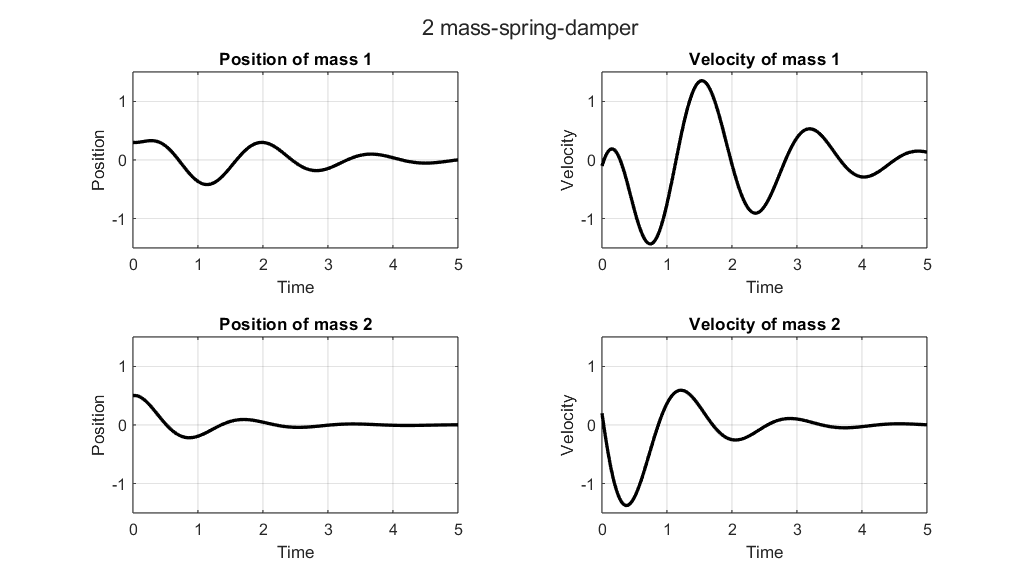
\includegraphics[width=0.9\linewidth]{report/Figures/system-response.png}
        \caption{Time response of a double mass-spring-damper system calculated using Equation \eqref{eqn:jordan-form-exponential}.}
        \label{fig:system-response}
    \end{figure}
\end{example}

If the matrix $A$ is not stable, but stability properties are still desired. The control law
\begin{equation}\label{eqn:feedback-control-law}
    u = Kx \implies x = Ax + BKx \implies \dot{x} = (A+BK)x
\end{equation}
can be used to stabilize the system, if and only if the system \eqref{eqn:standard-noiseless-system} is stabilizable \cite[Theorem 14.5]{Hespanha2018LinearTheory}. As can be seen in Equation \eqref{eqn:feedback-control-law}, the control law requires measuring the full state $x$, which can be very costly or not possible to measure \cite{yappa}. Figure \ref{fig:feedback-diagram} shows a simple feedback controlled system, where it can also be seen that $y$ feeds into the controller and can thus only stabilize the system when $y=x$. So we will now work towards creating a state estimate $\hat{x} \rightarrow x$ as $t \rightarrow \infty$.

\begin{figure}[H]
    \centering
    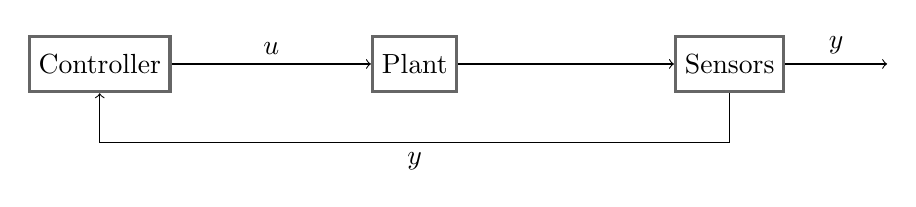
\begin{tikzpicture}[
        block/.style={rectangle, draw=black!60, very thick, minimum size=7mm},
        ]
        \node (plant) at (0,0) [block] {Plant};
        \node (sensors) at (4,0) [block] {Sensors};
        \node (controller) at (-4,0) [block] {Controller};

        \draw[->] (plant) -- (sensors);
        \draw[->] (sensors) -- node[auto] {$y$} (6,0);
        \draw[->] (sensors) -- (4,-1) -- node[auto] {$y$} (-4,-1) -- (controller);
        \draw[->] (controller) -- node[auto] {$u$} (plant);
        
    \end{tikzpicture}
    \caption{Feedback control system}
    \label{fig:feedback-diagram}
\end{figure}
 
\subsection{Observability}
We now aim to reconstruct the full state $x$ from the output $y$ and the input $u$. The following derivation is based on \cite{StephenBoyd2009LectureEstimation}, consider system \eqref{eqn:standard-noiseless-system} where $x$ is unknown and $y$ and $u$ are known. The derivatives of $y$ 
\[
\begin{split}
y &= Cx + Du \\
\dot{y} &= C\dot{x} + Du =  CAx + CBu + D\dot{u} \\
\Ddot{y} &= CA\dot{x} + CBu + Du = CA^{2}x + CABu + CB\dot{u} + D\Ddot{u} \\
\vdots \\
y^{(n_x)} &= CA^{n_x}x + CA^{n_x-1}Bu + CA^{n_x-2}B\dot{u} + \dots + CABu^{(n_x-2)} + CBu^{(n_x-1)} + Du^{(n_x)}
\end{split}
\]
will be used to reconstruct $x$ from the derivatives of $y$ and $u$. These derivatives of $y$ can be combined into
\[ \mathbf{y} =  \mathcal{O}x + \mathcal{K}\mathbf{u}
,\]
where
\[\mathbf{y}=
\begin{bmatrix}
    y \\
    y^{(1)} \\
    y^{(2)} \\
    \vdots \\
    y^{(n-1)} \\
\end{bmatrix} \quad \text{and} \quad
\mathbf{u} = 
\begin{bmatrix}
    u \\
    u^{(1)} \\
    u^{(2)} \\
    \vdots \\
    u^{(n-1)} \\
\end{bmatrix},
\]
are vectors containing the derivatives of the output and the input,
\begin{equation}\label{eqn:observability-matrix}
    \mathcal{O}=
    \begin{bmatrix}
        C \\
        CA \\
        CA^2 \\
        \vdots \\
        CA^{n-1}
    \end{bmatrix}    
\end{equation}

is the \textit{observability matrix} and
\[ \mathcal{K}=
\begin{bmatrix}
    D & 0 & 0 & \hdots & 0\\
    CB & D & 0 & \hdots & 0\\
    CAB & CB & D & \hdots & 0 \\
    \vdots & \vdots & \vdots & \ddots & \vdots \\
    CA^{n-2}B & CA^{n-3}B & CA^{n-4}B & \hdots & D
\end{bmatrix}.
\]
Isolating $x$ results in
\begin{equation}\label{eqn:state-estimation-w-observability-matrix}
    x = \mathcal{O}^{-1}(\mathbf{y}-\mathcal{K}\mathbf{u}).
\end{equation}
As can be seen in \eqref{eqn:state-estimation-w-observability-matrix} observability matrix $\mathcal{O}$ is required to be invertible to reconstruct $x$ from the time derivatives of $y$ and $u$. If a system's $A$ and $C$ matrix fulfil this requirement, the system can be described as \textit{observable}. The invertibility requirement is equivalent to the statement that the matrix $\mathcal{O}$ needs to be full rank \cite[Section 2.9]{Lay2016LinearApplications}, this theorem that can also be found in \cite[Corollary 3.8]{Antsaklis2006LinearSystems}. The implication of this is that it is only possible to reconstruct the state $x$ if the pair $(A,C)$ is observable. 

\begin{example}\label{ex:single-ouptut-observability}
    Let us work out an example on the system presented in Example \ref{ex:system} where only the position of the first mass is measured. This leads to the following system matrices:
\begin{equation*}
    A =
    \begin{bmatrix}
        0 & 1 & 0 & 0 \\
        -15 & -2 & 15 & 2 \\
        0 & 0 & 0 & 1 \\
        0 & 0 & -15 & -2 \\
    \end{bmatrix}, \quad
    C =
    \begin{bmatrix}
        1 & 0 & 0 & 0 \\
    \end{bmatrix}.
\end{equation*}
We now compute the observability matrix
\begin{equation*}
    \mathcal{O} = 
    \begin{bmatrix}
        C \\ CA \\ CA^2 \\ CA^3 \\
    \end{bmatrix} =
    \begin{bmatrix}
        1 & 0 & 0 & 0 \\
        0 & 1 & 0 & 0 \\
        -15 & -2 & 15 & 2 \\
        30 & -11 & -60 & 7 \\
    \end{bmatrix}
\end{equation*}
which has rank $4$ and so the pair $(A,C)$ is observable.
\end{example}

Example \ref{ex:single-ouptut-observability} considers a system with only one output, we will now investigate the case with multiple outputs. Let us expand the observability matrix \eqref{eqn:observability-matrix} for a system where $n_y>1$, a system with more than one output.
\begin{equation*}
\mathcal{O}=
\begin{bmatrix}
    C \\
    CA \\
    \vdots \\
    CA^{n-1}
\end{bmatrix}    
=
\begin{bmatrix}
    c_1 \\
    \vdots \\
    c_{n_y} \\
    c_1A \\
    \vdots \\
    c_{n_y}A \\
    \vdots \\
    c_1A^{n-1}\\
    \vdots \\
    c_{n_y}A^{n-1} \\
\end{bmatrix}_{n_xn_y \times n_x}.
\end{equation*}
The same rank condition still holds, the system is fully observable as long as the $\mathcal{O}$ matrix is full rank. This implies that certain combinations of sensors that do not suffice on their own can make a system fully observable \cite[Section 3.4 D 2]{Antsaklis2006LinearSystems}.
\textcolor{red}{how does observability matrix lead to the observer}
\subsection{Single observer}
Let us now reconstruct the full state of system \eqref{eqn:standard-noiseless-system} from  $y$ and $u$ by defining the state estimate as in \cite[Section 16.5]{Hespanha2018LinearTheory}
\begin{equation}\label{eqn:stable-simple-state-estimator}
    \dot{\hat{x}} = A\hat{x} + Bu, \quad \hat{y} = C\hat{x} + Du.
\end{equation}
We now define the \textit{state estimation error}
\begin{equation}\label{eqn:estimate-error}
    e = \hat{x} - x
\end{equation}
which we differentiate and substitute equations \eqref{eqn:standard-noiseless-system} and \eqref{eqn:stable-simple-state-estimator} into to give
\begin{equation*}
    \dot{e} = \dot{\hat{x}} - \dot{x} = A\hat{x} + Bu - Ax - Bu = Ae.
\end{equation*}
We can now conclude that $e \rightarrow 0$ as $t \rightarrow \infty$ if the matrix $A$ is a stability matrix. Let us now define a state estimator that provides an asymptotically correct state estimate even when $A$ is not a stability matrix as in \cite[Section 16.5]{Hespanha2018LinearTheory}
\begin{equation}\label{eqn:unstable-simple-state-estimator}
    \dot{\hat{x}} = A\hat{x} + Bu + L(\hat{y} - y), \quad \hat{y} = C\hat{x} + Du.
\end{equation}
We now perform the same analysis on the derivative of the state estimation error
\begin{equation}\label{eqn:error-linear-observer}
    \dot{e} = A\hat{x} + Bu + L(C\hat{x} + Du - Cx - Du) - Ax - Bu = (A+LC)e
\end{equation}
which is similar to the solution in \eqref{eqn:zero-input-solution}. From which we can conclude that if $A+LC$ is a stability matrix $e \rightarrow 0$ as $t \rightarrow \infty$. Figure \ref{fig:observer-diagram} shows the observer placed between the sensors and the controller

\begin{figure}[ht]
    \centering
    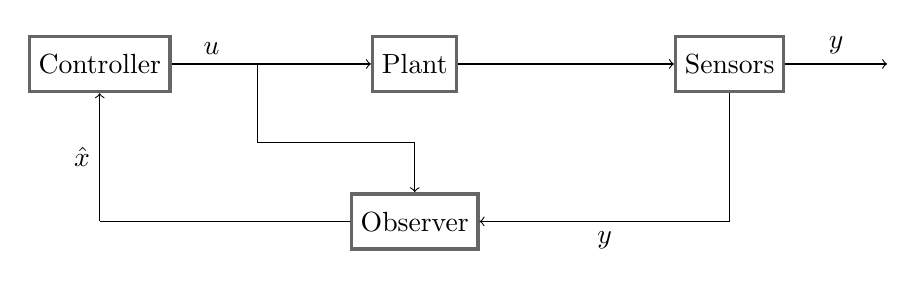
\begin{tikzpicture}[
        block/.style={rectangle, draw=black!60, very thick, minimum size=7mm},
        ]
        \node (plant) at (0,0) [block] {Plant};
        \node (sensors) at (4,0) [block] {Sensors};
        \node (observer) at (0,-2) [block] {Observer};
        \node (controller) at (-4,0) [block] {Controller};

        \draw[->] (plant) -- (sensors);
        \draw[-] (sensors) -- (4,-2);
        \draw[->] (4,-2) -- node[auto] {$y$} (observer);
        \draw[->] (sensors) -- node[auto] {$y$} (6,0);
        \draw[-] (observer)  -- (-4,-2);
        \draw[->] (-4,-2) -- node[auto] {$\hat{x}$} (controller);
        \draw[->] (controller) -- node[pos=0.2,above] {$u$} (plant);
        \draw[->] (-2,0) -- (-2,-1) -- (0,-1) -- (observer);
    \end{tikzpicture}
    \caption{An observer in a control system}
    \label{fig:observer-diagram}
\end{figure}

It is important to note that no restrictions are set on the structure of $y$ and therefore $C$ as long as the pair $(A,C)$ is observable. 

Let us now extend the observer \eqref{eqn:unstable-simple-state-estimator} to also correctly estimate systems with a nonlinear contribution $\phi(x)$. Consider the system
\begin{equation*}\label{eqn:nonlinear-system}
    \dot{x} = Ax + Bu + E\phi(y), \quad y = Cx + Du.
\end{equation*}
The observer will be constructed as
\begin{equation}\label{eqn:nonlinear-single-observer}
    \dot{\hat{x}} = A\hat{x} + Bu + E\phi(y) + L(\hat{y} - y), \quad \hat{y} = C\hat{x} + Du.
\end{equation}
Note that the input to the nonlinearity is $y$. Let us now substitute these definitions into the derivative of the error $e=\hat{x}-x$
\begin{equation*}\label{eqn:errror-nonlinear-observer}
    \begin{split}
        \dot{e} = \dot{\hat{x}} - \dot{x} &= A\hat{x} + Bu + E\phi(y) + L(\hat{y} - y) - Ax - Bu - E\phi(y) \\
        &= (A+LC)e + E(\phi(y) - \phi(y)) \\
        &= (A+LC)e.
    \end{split}
\end{equation*}
It is now evident why $\phi(y)$ is used in equation \eqref{eqn:nonlinear-system}, otherwise $e \rightarrow 0$ as $t \rightarrow \infty$ cannot be guaranteed. Because $\phi(y)$ does not necessarily equal $\phi(x)$, $\phi(y) - \phi(x)$ does not necessarily equal $0$. This does set certain requirements on $y$, variables that affect the nonlinearity need to be measured directly. For the multi mass-spring-damper system as in Chapter \ref{ch:system-definition} this means that all positions $x_a,a=1,2,\dots,b$ need to be measured directly. 

\subsection{Eigenvalue placement}
Since we have full control over $L$, we will now discuss methods to place eigenvalues of $A+LC$ at desired locations and what constraints are limiting our control over these eigenvalues.

\begin{theorem}[Observer eigenvalues]
\label{th:arbitrary-alc-eigenvalues}
    If the pair $(A,C)$\eqref{eqn:standard-noiseless-system} is observable there exists an $L \in \mathbb{R}^{n \times m}$ that influences all eigenvalues of $A+LC$.
\end{theorem}
\begin{proof}
    This proof is based on \cite[Section 4.2]{Antsaklis2006LinearSystems}. Suppose that the pair $(A,C)$ is not fully observable and that all eigenvalues of $A+LC$  have been influenced by $L$, it will be shown that this leads to a contradiction. There exists a similarity transformation that separates the observable from the unobservable part: the observable decomposition \cite[Section 16.1]{Hespanha2018LinearTheory}. Specifically there exists a matrix $Q$ that
    \begin{equation}
    \begin{split}
        Q^{-1}(A+LC)Q 
        &= Q^{-1}AQ + Q^{-1}LCQ =
        \begin{bmatrix}
            A_o & 0 \\
            A_{21} & A_u
        \end{bmatrix}
        + 
        \begin{bmatrix}
            L_1 \\
            L_2
        \end{bmatrix}
        \begin{bmatrix}
            C_o & 0
        \end{bmatrix} \\
        &=
        \begin{bmatrix}
            A_o + L_1 C_o & 0 \\
            A_{21} + L_2 C_o & A_u
        \end{bmatrix}
    \end{split}
    \end{equation}  
where the pair $(A_o,C_o)$ is observable. A similarity transformation leaves the eigenvalues unchanged \cite[Section 5.2]{Lay2016LinearApplications}. The lower triangular structure of the matrix implies that the eigenvalues of $A_u$ remain the same, which leads to a contradiction: not all the eigenvalues of $A+LC$ have been influenced. Thus, if the pair $(A,C)$ is observable there exists an $L$ that can influence all eigenvalues of $A+LC$.
\end{proof}
\textcolor{red}{remove proof}

An analytical method to place the eigenvalues at arbitrary locations in a MIMO system is presented in \cite[Section 4.2 B]{Antsaklis2006LinearSystems}, where the system is first transformed into \textit{observer form} by a similarity transformation. After this transformation the deriving the matrix $L$ is convenient. Another option is numerically deriving $L$. Matlab provides the function \texttt{place}, based on the algorithm presented in \cite{Kautsky1985RobustFeedback}.

\textcolor{red}{Unsatisfying conclusion, would prefer to show an actual strategy to choose the eigenvalues.}

\subsection{\textcolor{red}{what eigenvalues to choose}}


